\documentclass{article}

\usepackage{amsmath, amsthm, amssymb, amsfonts}
\usepackage{thmtools}
\usepackage{graphicx}
\usepackage{setspace}
\usepackage{geometry}
\usepackage{float}
\usepackage{hyperref}
\usepackage[utf8]{inputenc}
\usepackage[english]{babel}
\usepackage{framed}
\usepackage[dvipsnames]{xcolor}
\usepackage{tcolorbox}

\newcommand{\HRule}[1]{\rule{\linewidth}{#1}}

% ------------------------------------------------------------------------------

\begin{document}

% ------------------------------------------------------------------------------
% Cover Page and ToC
% ------------------------------------------------------------------------------

\title{ \normalsize \textsc{}
		\\ [2.0cm]
		\HRule{1.5pt} \\
		\LARGE \textbf{Parallel and Distributed Computing
		\HRule{2.0pt} \\ [0.6cm] \LARGE{Project Report - OpenMP Delivery} \vspace*{10\baselineskip}}
		}
\date{}
\author{\textbf{Authors} \\ 
		Carolina Coelho - 99189\\
		Diogo Melita - 99202\\
		Diogo Antunes - 99210}

\maketitle
\newpage

% ------------------------------------------------------------------------------

\section{Introduciton}

For this stage of the project, we were asked to optimize our 
serial version using OpenMP. We will be using the same 
implementation as the previous stage, but we will be adding 
OpenMP directives to parallelize the code. 

\section{Serial Version}

The serial version of the code was already implemented in the previous
stage of the project. However, we modified some parts of the code because 
we realized that this would make it more optimized.

First, we created a \texttt{prepare} function that initializes a new grid and 
the vectors common to all generations, and a \texttt{finish} function that 
prints the results. These functions were called outside the \texttt{simulation} 
function, as they are not counted in the execution time.

The original code utilizes nested loops to iterate over a specified neighborhood 
range, checking each neighboring cell and updating counts accordingly. 
However, the modified version directly accesses specific neighboring cells without 
the need for nested loops. Each neighbor of the current cell is explicitly accessed 
and counted. This change reduced redundant calculations and improved data locality.

\section{Approach Used}

The first step was to identify the parts of the code that 
could be parallelized. By analyzing the code, we concluded that 
the most time-consuming part was on the function \texttt{simulation}. 
This function is responsible for simulating the multiple generations, 
and therefore, it is very time consuming.

Upon identifying the part of the code that could be parallelized, 
we identified the 2 nested loops that needed to be took care of in 
order to speed up the code: the nested loop that calculates the initial statistics 
of the grid and the loop that calculates the next generation of the grid. 

Additionally, we also used \textbf{VTune} to profile the code and 
identify the most time-consuming parts of the code in order to ease 
the parallelization process.

\section{OpenMP Parallelization}
To parallelize the code, we used the OpenMP directives, more specifically  
the following directives: \texttt{parallel}, \texttt{for}, \texttt{collapse}, 
\texttt{reduction}, and \texttt{single}.

The \texttt{parallel} directive is used to create a team of threads 
that will execute the code inside the block. In this block, we have 
all the code mentioned above that we wanted to parallelize.

To parallelize the loops, we combined the \texttt{for}, \texttt{collapse}, 
and \texttt{reduction} directives. The \texttt{for} directive is used to parallelize
different iterations of the loop among the threads. The \texttt{collapse} directive is used to collapse 
nested loops into one, in this case we used it to collapse the 3 loops since the grid is 3 dimentional.
Finally, the \texttt{reduction} directive is used to perform a reduction 
operation on the variables that are shared between the threads. In this case, we 
used this directive with the \texttt{+} operator to sum the number of cells of each 
specie in the new generations grid. Since the parallelization we intended to do was having 
multiple threads not only calulating the next generation of the grid, but also the 
number of cells of each specie we used the \texttt{reduction} directive as it 
makes a private copy for each thread of the variable specified and then combines 
the results at the end, thus achieving the intended result. 

Finally, we used the \texttt{single} directive to make sure that only one thread 
executed parts of the code inside the block that shouldn't be parallelized. This 
parts were responsible for swapping the pointers of the old and new grids and updating 
the maximum population of each specie and therefore, it was important to make sure that only 
one thread executed this part of the code to achieve the correct results.

\section{Results}

To test the parallelized code, we used the input files available on the course's page 
and the lab's machines. We were also careful to run the OpenMP version with the 
environment variable \texttt{OMP\_NUM\_THREADS} set to 1, 2, 4, and 6 in order to correctly 
test the speedup of our program. 

We compared the results of the parallelized code with the serial version and 
concluded that the parallelized version was much faster than the serial one. 
The speedup achieved was significant and close to the ideal speedup, the number of 
physical cores.

In the following table, we present the times of execution of the serial and parallelized 
versions of the code against the inputs available on the course page as well as the achieved 
speedup. This results were obtained by running both the serial and omp versions on the 
\textbf{lab3p8} machine, which has 6 physical cores. The omp version was ran with the 
\texttt{OMP\_NUM\_THREADS} environment flag set to 1, 2, 4, and 6.

\begin{table}[h!]
	\centering
	\begin{tabular}{||c c c c c c c||} 
	 \hline
	 Version & Number of Threads & Input 1 & Input 2 & Input 3 & Input 4 & Speedup\\ [0.5ex] 
	 \hline\hline
	 serial & $N/A$ & 9.5 & 15.0 & 48.7 & 115.5 & $N/A$ \\ 
	 omp & 1 & 9.4 & 15.0 & 48.3 & 115.2 & 1.0 \\ 
	 omp & 2 & 4.8 & 7.6 & 24.6 & 58.8 & 1.98 \\
	 omp & 4 & 2.5 & 3.9 & 12.6 & 30.1 & 3.84 \\
	 omp & 6 & 1.7 & 2.7 & 8.6 & 20.6 & 5.61 \\ [1ex] 
	 \hline
	\end{tabular}
	\caption{Times of execution, in seconds, of the serial and parallelized versions of the code.}
	\label{table:1}
\end{table}

\begin{table}[h!]
	\centering
	\begin{tabular}{||c c c c c||} 
	 \hline
	 Input & gen\_count & $N$ & density & seed  \\ [0.5ex] 
	 \hline\hline
	 1 & 1000 & 64 & 0.4 & 0 \\ 
	 2 & 200 & 128 & 0.5 & 1000 \\
	 3 & 10 & 512 & 0.4 & 0 \\ 
	 4 & 3 & 1024 & 0.4 & 100 \\ [1ex] 
	 \hline
	\end{tabular}
	\caption{Inputs used}
	\label{table:2}
\end{table}

In the graph below, we present the speedup achieved by the parallelized version 
when running on different number of threads. As we can see, the speedup achieved 
is significant and close to the ideal speedup. Our tests were run multiple times 
and the results were consistent.

\begin{figure}[htbp]
    \centering
    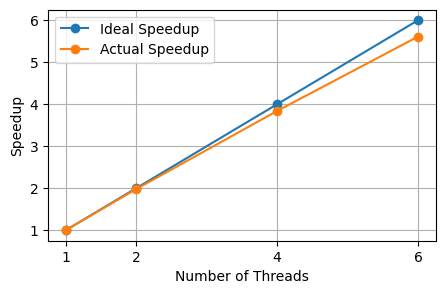
\includegraphics[width=0.5\textwidth]{img/speedup-threads.png}
    \caption{Speedup achieved by the parallelized version when running on different number of threads.}
    \label{fig:name}
\end{figure}

\newpage

% ------------------------------------------------------------------------------
% Reference and Cited Works
% ------------------------------------------------------------------------------

\bibliographystyle{IEEEtran}
% \bibliography{References.bib}

% ------------------------------------------------------------------------------

\end{document}
